\section{Key-Value DataBase Implementation}

\subsection{Technologies used: LevelDB}

To implement our key-value database we used \specialname{LevelDB}, a library
written at Google that provides a fast key-value persistent data storage engine.

More precisely we used the Java porting of \specialname{LevelDB} packaged as
\code{org.iq80.leveldb}, which have full code available on \specialname{GitHub}.

\lstinputlisting[language=XML, style=xmlcode, label={lst:pomleveldb},
caption={Maven dependency for LevelDB.}]{pomleveldb.xml}

This database can be used only via its API, that provides a tiny set of basic
operations (put, get, delete) that we can exploit to implement more complex
functions.

Furthermore it provides snapshots, support for atomic operations and
an iterator to allow us to flow among the entries and examine them one at a
time.

\subsection{UML Implementation Diagram}

In Figure~\ref{fig:serverkvdb} is shown the diagram where we can see the classes
that have been implemented to introduce the Key Value database in the
application.

The classes have been packaged inside \code{ristogo.server.storage.kvdb}.

\begin{landscape}
	\begin{figure}
		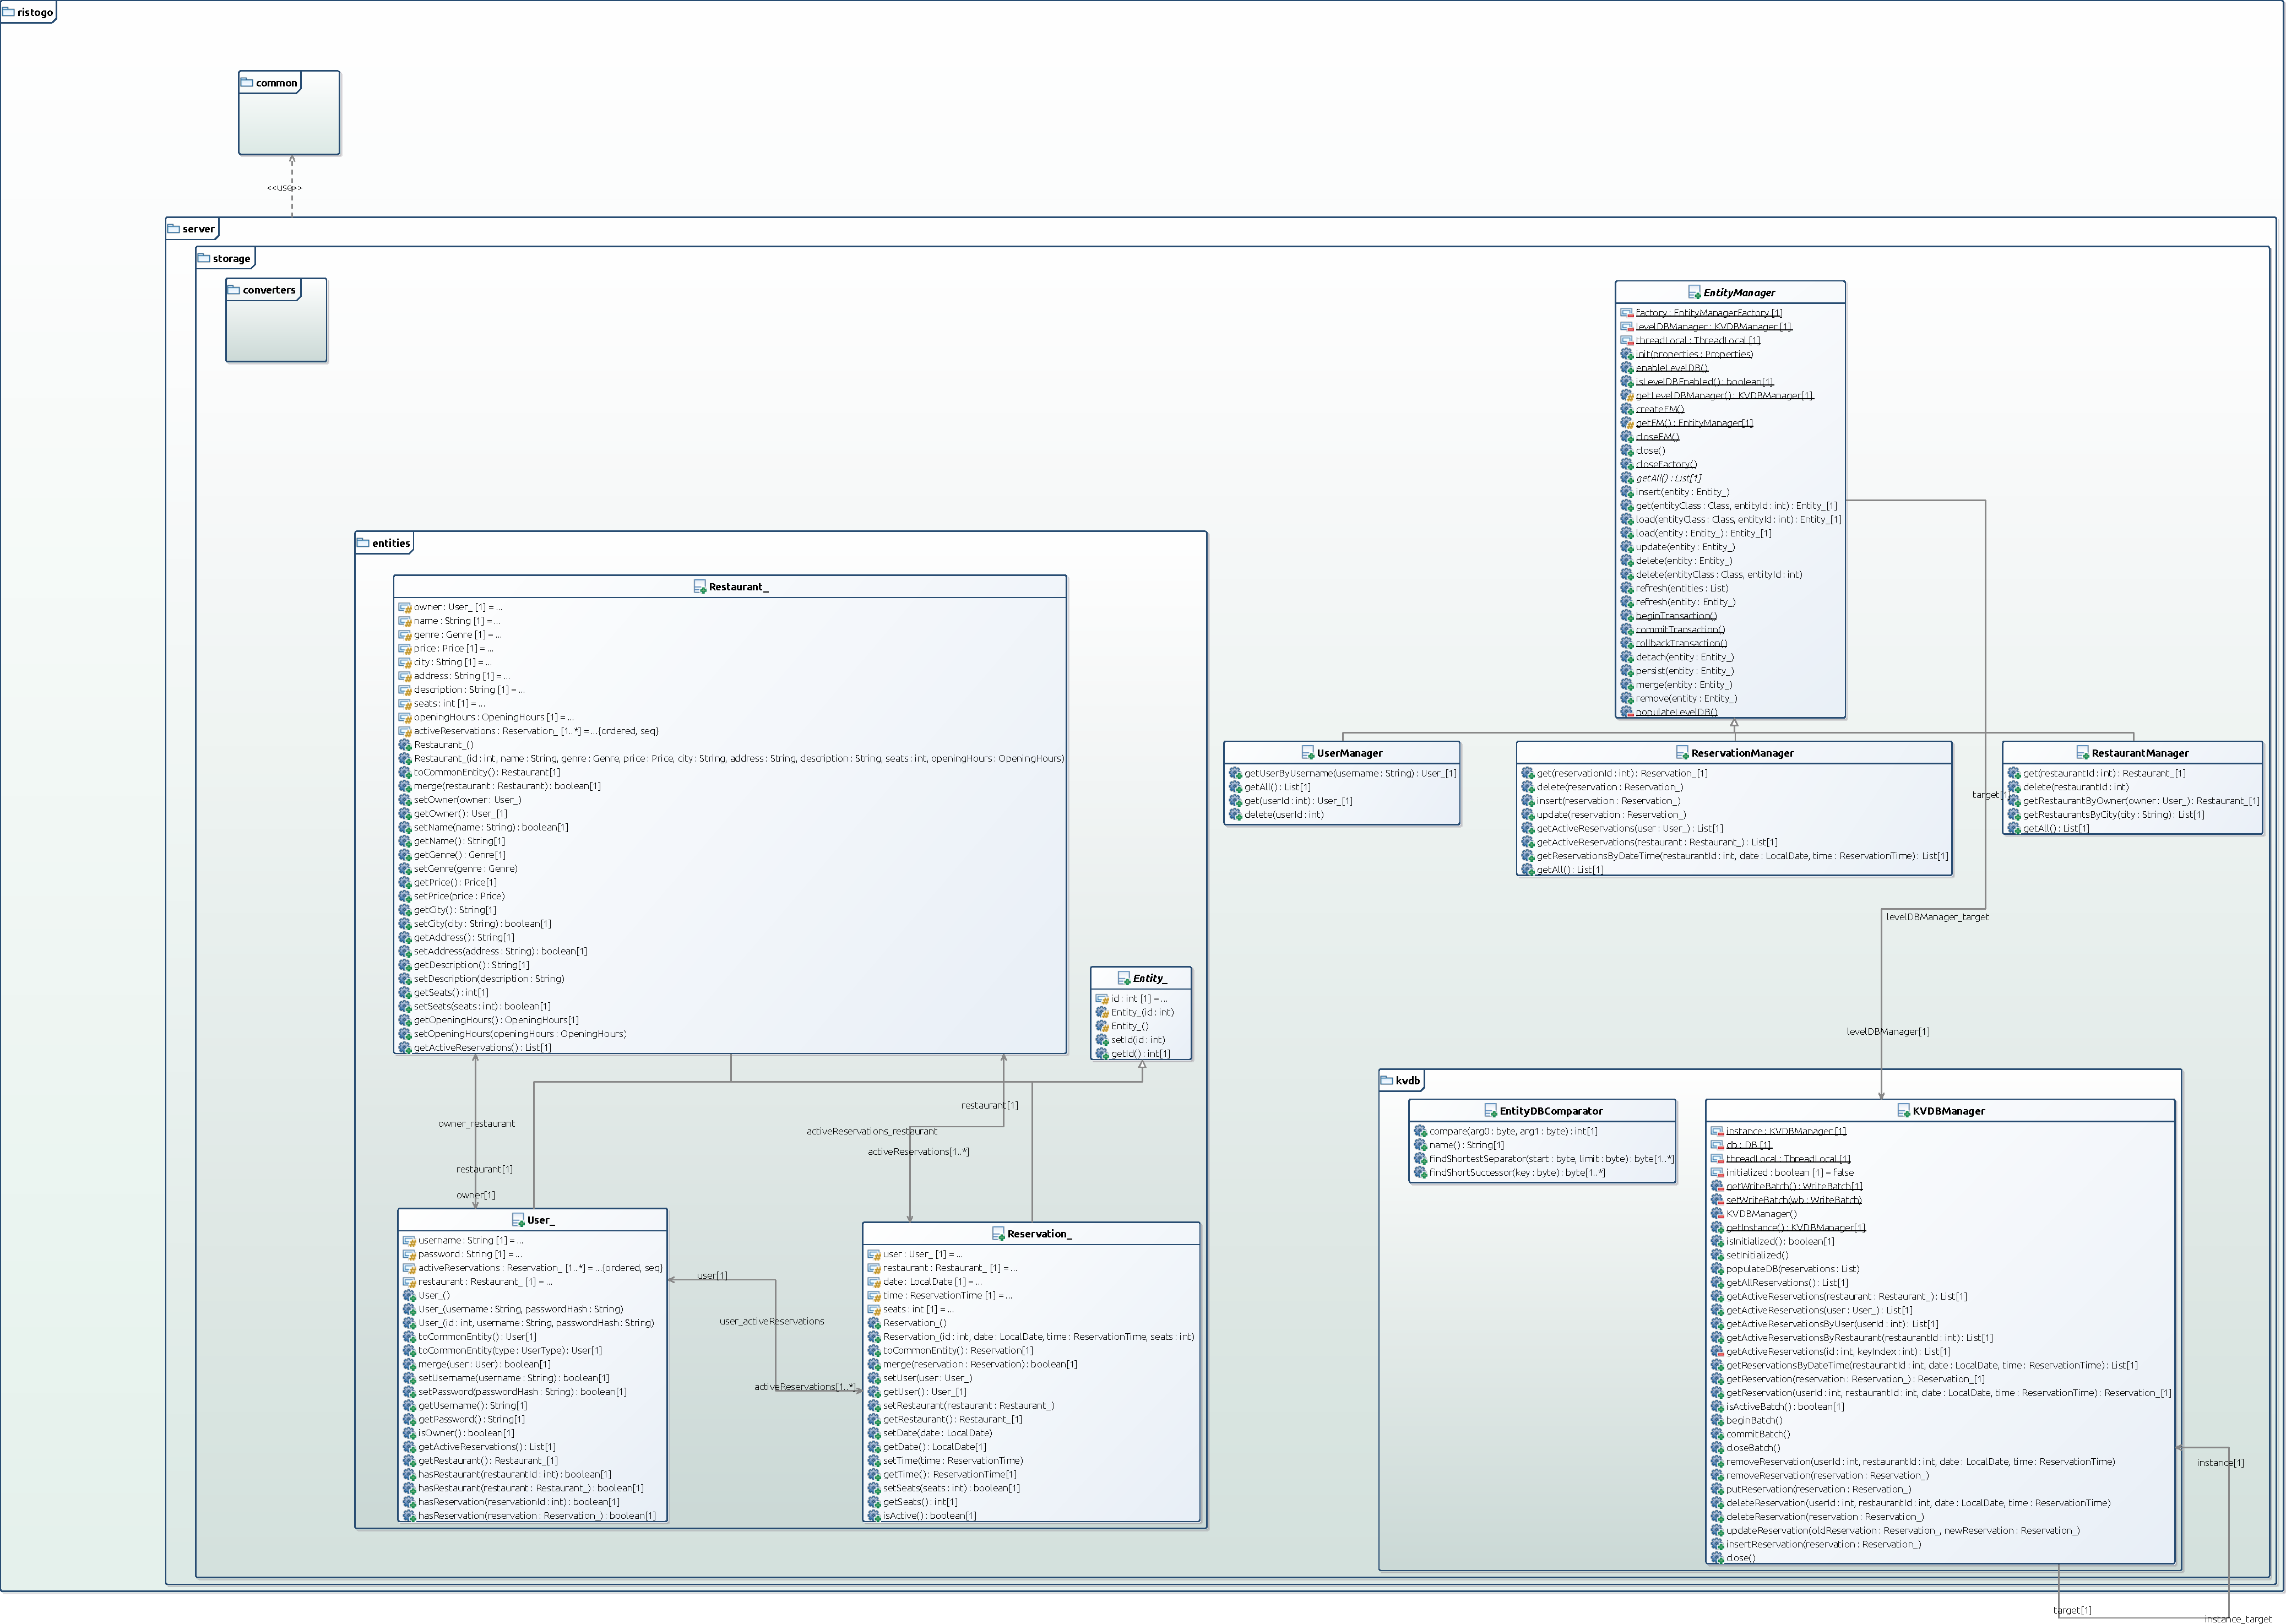
\includegraphics[width=0.70\paperheight]{serverkvdb.pdf}
		\caption{\code{ristogo.server.storage.kvdb} UML Implementation Diagram.}
		\label{fig:serverkvdb}
	\end{figure}
\end{landscape}

The behaviour of this datastore is as described previously.

When the server application starts it builds the key value database starting
from the data present in the relational database. This operation is performed
just if the key-value database (from now shortened as kvdb) is not present in
the system, then the application will manage the synchronization among the two
databases, keeping the consistency.

When a request arrives at the server, if this request implies a read operation
the \code{EntityManager} involved read will from the kvdb.

If instead the request implies a write operation it is handled in a
write-through fashion. The \code{EntityManager} involved will write into the
kvdb and into the relational database.
